\documentclass[a4paper,12pt]{article}
\usepackage[T1]{fontenc}
\usepackage[utf8]{inputenc}
\usepackage{graphicx}
\usepackage{amsmath}
\usepackage{amsfonts}
\usepackage{amssymb}
\usepackage{booktabs}
\usepackage{float}
\usepackage{geometry}
\usepackage[ngerman,provide=*]{babel}
\usepackage{enumitem}
\usepackage{parskip}
\usepackage{underscore}
\usepackage{hyperref}
\usepackage{multicol}

\geometry{a4paper, left=25mm, right=25mm, top=20mm, bottom=20mm}

%%%%%%%%%%%%%%% Titelblatt %%%%%%%%%%%%%%%
\begin{document}
\begin{titlepage}
    \centering
    
\includegraphics[scale = 0.03]{bilder/JKU_Logo.png}\\[1.0 cm]	% JKU Logo
    \textsc{\Large Einführungspraktikum Physik}\\[0.5 cm]	        % LVA Name
    \textsc{\large 2. Versuch}\\[0.5 cm]				            % Versuch Nummer    // [x] TODO: Versuch Nummer anpassen
    \rule{\linewidth}{0.4 mm} \\[0.4 cm]
    { \huge \bfseries Reaktionszeit}\\                              % Versuch Name      // [x] TODO: Versuch Name anpassen
    \rule{\linewidth}{0.4 mm} \\[1.5 cm]
    \begin{minipage}{0.8\textwidth}
        \begin{flushleft} \large
            \emph{Autoren:}\\
            Eva Brandstätter (k12406599)\\
            Tobias Mittermair (k12412801)\\
            \vspace{1cm}
            \emph{Gruppe:}\\
            Freitag Vormittag\\
            \vspace{1cm}
            \emph{Betreuer:}\\
            Gerald Gmachmeir
        \end{flushleft}
        \begin{flushright} \large
            \vspace{8cm}
            \emph{Abgabe:} \\
            \today
        \end{flushright}
    \end{minipage}~    
\end{titlepage}

%%%%%%%%%%%%%%% Inhaltsverzeichnis %%%%%%%%%%%%%%%
\tableofcontents
\newpage


%%%%%%%%%%%%%%% Inhalt %%%%%%%%%%%%%%%
\section{Einleitung}
%//[x] TODO: Einleitung
% Was soll gemessen werden? (Ziel / Motivation / Hypothese / erwartetes Ergebnis)

Die Reaktionszeit einer Experimentatorin kann Einfluss auf Versuchsergebnisse haben. Daher ist es wichtig,
diese zu kennen und zu verstehen.

In diesem Experiment wird die mittlere Reaktionszeit einer Probandin (Eva Brandstätter) sowie die Verteilung 
der Reaktionszeit ermittelt. Außerdem soll näher auf deren statistische Größen und Verteilungen
eingegangen werden.

Es wird vermutet, dass die Reaktionszeit annähernd Normalverteilt ist. Die gemessene Größe, aus der die
Reaktionszeit ermittelt wird (Länge), ist aber nicht direkt proportional zur Zeit. Deshalb wird die 
Hypothese aufgestellt, dass die Verteilung dieser Größe nicht mehr einer Gaußverteilung entspricht (verzerrt ist).

Weiters soll deshalb behandelt werden, ob und wieso es einen Unterschied zwischen mittleren Zeit und
der Zeit aus der gemittelten Länge gibt.

\section{Grundlagen}
%//[x] TODO: Grundlagen
% (kurz!) Was muss ich über die zu messende Größe wissen?

Als Reaktionszeit bezeichnet man die Zeit, die vergeht von einem auslösenden Ereignis bis zu einer Reaktion seitens der zu Testenden.
In diesem Versuch wird dabei die Fallstrecke $h_i$ gemessen, die das Lineal zurücklegt, bevor es von der zu Testenden gefangen wird.
Der Index $i$ steht dabei für den $i$-ten Messwert.  
Aus dieser Strecke berechnet man sich mit der folgenden Formel die Reaktionszeit von der zu Testeden.

\begin{equation}
    t_i = \sqrt{\frac{2 \cdot h_i}{g}}
\end{equation}

Dabei ist $g$ die Erdbeschleunigung, die in diesem Versuch mit $9.81 \frac{m}{s^2}$ angenommen wird und deren Unsicherheit
vernachlässigt wird. 

Die Reaktionszeit kann durch verschiedene Faktoren beeinflusst werden. Nennenswert hierfür ist der Lidschlag (der die Sehfähigkeit 
für eine kurze Zeit unterbricht) oder die körperliche Verfassung sowie die Konzentrationsfähigkeit der zu testenden Person.

Für die statistischen Größen werden folgende Formeln verwendet:

\begin{equation}
    \label{eq:mittelwert}
    \mu = \frac{1}{N} \sum_{i=1}^{N} x_i
\end{equation}

\begin{equation}
    \label{eq:standardabweichung}
    \sigma = \sqrt{\frac{1}{N} \sum_{i=1}^{N} (x_i - \mu)^2}
\end{equation}

\begin{equation}
    \label{eq:standardabweichungDesMittelwerts}
    \sigma_\mu = \frac{\sigma}{\sqrt{N}}
\end{equation}

\newpage

Mithilfe der Fehlerfortpflanzung kann die Unsicherheit der Fallstrecke auf die Reaktionszeit
umgerechnet werden. Da die Messungen unkorreliert sind, kann man die Gauß'sche Fehlerfortpflanzung
verwenden:

\begin{equation}
    \label{eq:GaußFehlerfortpflanzung}
    \sigma_t = \sqrt{\left(\frac{\partial t}{\partial h} \cdot \sigma_h\right)^2}
\end{equation}


\section{Versuchsbeschreibung}
\subsection{Versuchsaufbau}
%//[x] TODO: Versuchsaufbau
% Wie sieht der Versuchsaufbau aus? (Skizze, Anleitung, Geräte, …)
% auf Abbildungen Bezug nehmen

Für den Versuch wurde sowohl ein 30cm-Lineal als auch ein Millimeterpapier zur Verfügung gestellt. Weiters stand ein 
Laptop zur Führung des Laborprotokolls bereit und zur Dokumentation der Werte.

\subsection{Durchführung}
%//[x] TODO: Durchführung
% Wie wurde der Versuch durchgeführt bzw. ausgewertet?
% auch wann und wo?

Der Versuch wurde am 22. November 2024 im Raum P122 an der JKU in Linz durchgeführt. Es wurden 138 Messpunkte erfasst.

Der "Tester" (Tobias Mittermair) hält das Lineal senkrecht zum
Boden, möglichst ohne zu zittern. Um dies zu gewährleisten, wurden die zwei Finger, die das Lineal hielten, von 
der anderen Hand gestützt. Die Versuchsperson (die "zu
Testende") platziert ihre Hand an der 0cm-Markierung, sodass an der Oberkante des Daumens die 0cm-Markierung 
abgelesen werden kann. Dabei wird der Abstand zwischen den Fingern möglichst gering gewählt (ohne das Lineal zu 
berühren), sodass beim Durchfallen des Lineals dieses schnell gefasst werden kann.

Nun lässt der Tester das Lineal möglichst unvorhersehbar für die andere Person los und die zu Testende fängt es 
so schnell es ihr möglich ist.
Danach wird die Länge am Lineal and der Oberkante des Daumens abgelesen und in
die Tabelle eingetragen. Weiters wird nebenbei ein Histogramm auf einem Millimeterpapier
angefertigt.

Es ist einerseits darauf zu achten, dass es vom "Tester" keinerlei Signal gibt, dass das Lineal
fallengelassen wird. Andererseits soll das Lineal immer in ungefähr der gleichen Position vom Tester zur Probandin
gehalten werden.

\section{Messergebnisse und Auswertung}
\subsection{Messwerte und Unsicherheiten}
%//[x] TODO: Messung - evtl. nur Verweis auf Messergebnisse
% Eigentliche Messung!
% Wie groß sind die Messunsicherheiten („Messfehler“)?

Die Messwerte sind dem Anhang (Kapitel \ref{AnahangFallstrecke}) zu entnehmen. 

Bezüglich den Messunsicherheiten unterscheidet man bei den abgelesenen Messwerten die 
Skalenunsicherheit des Lineals und der Unsicherheit des Daumens 
Die Skalenunsicherheit (übersetzt auf normalverteilt) beträgt $\pm \frac{0.5}{\sqrt{3}}\mathrm{mm}$,
welche man in Anbetracht der Ableseunsicherheit vernachlässigen kann, da diese auf $\pm 3\mathrm{mm}$
geschätzt wird. In diese Unsicherheit fließen Faktoren ein, wie die Perspektive
und die Auflagefläche des Daumens, die sich je nach ausgeübter Kraft beim Zugreifen variiert.
Deshalb wird $u_h \approx 3\mathrm{mm}$ gewählt.

\newpage

Da die Messungen unkorreliert sind, kann mithilfe der Gauß'schen Fehlerfortpflanzung
(Gl. \ref{eq:GaußFehlerfortpflanzung}) die Unsicherheit der Fallstrecke auf die Reaktionszeit umgerechnet werden

Die Ableitung der Reaktionszeit nach der Fallstrecke ergibt sich zu:

\begin{equation}
    \frac{\partial t(h)}{\partial h} = \frac{1}{\sqrt{2 \cdot g \cdot h}}
\end{equation}

Nun kann die Unsicherheit der Reaktionszeit berechnet werden:

\begin{equation}
    u_t(h) = \sqrt{\left(\frac{1}{\sqrt{2 \cdot g \cdot h}} \cdot u_h\right)^2}
\end{equation}

An dieser Formel ist zu erkennen, dass die Unsicherheit der Reaktionszeit mit steigender Fallstrecke abnimmt.
Beispielsweise für $h=h(\mu_t)$ ergibt sich $u_t(h(\mu_t)) \approx 0.0018\mathrm{s}$.


\subsection{Auswertung}
%//[x] TODO: Auswertung
% evtl. Formeln, etc.
% auf richtiges Runden der Werte achten
% evtl. auf Gleichungen Bezug nehmen

Der Mittelwert, die Standardabweichung und Standardabweichung des Mittelwerts wurden nach den
Gleichungen \ref{eq:mittelwert}, \ref{eq:standardabweichung} und \ref{eq:standardabweichungDesMittelwerts}
jeweils für die Fallstrecke $h$ und die Reaktionszeit $t$ berechnet:

\begin{table}[H]
    \centering
    \begin{tabular}{c c c}
        \parbox{4cm}{
            \begin{align*}
                \mu_h &= 14.42\mathrm{cm} \\
                \sigma_h &= 2.55\mathrm{cm} \\
                {\sigma_\mu}_h &= 0.22\mathrm{cm}
            \end{align*}
        } & \hspace{1cm} & \parbox{4cm}{
            \begin{align*}
                \mu_t &= 0.1708\mathrm{s} \\
                \sigma_t &= 0.0152\mathrm{s} \\
                {\sigma_\mu}_t &= 0.0013\mathrm{s}
            \end{align*}
        } \\
    \end{tabular}
\end{table}

Zusätzlich wurde überprüft, ob $t(\mu_h)\stackrel{?}{=}\mu_t$ ist:

\begin{align*}
    t(\mu_h) &= \sqrt{\frac{2 \cdot \mu_h}{g}} \\
    &= 0.1714\mathrm{s} \neq \mu_t
\end{align*}

Außerdem wurden Histogramme für Fallstrecke und Reaktionszeit angefertigt, um die Verteilung
der Messwerte zu visualisieren. Weiters sind in beiden Diagrammen entsprechende Normalverteilungskurven
eingezeichnet. Allerdings sei darauf hingewiesen, dass die Normalverteilungskurven nur als Referenz dienen.

% Diagramme der Auswertung
\begin{figure}[H]
    \label{Abb:HistogrammFallstrecke}
    \centering
    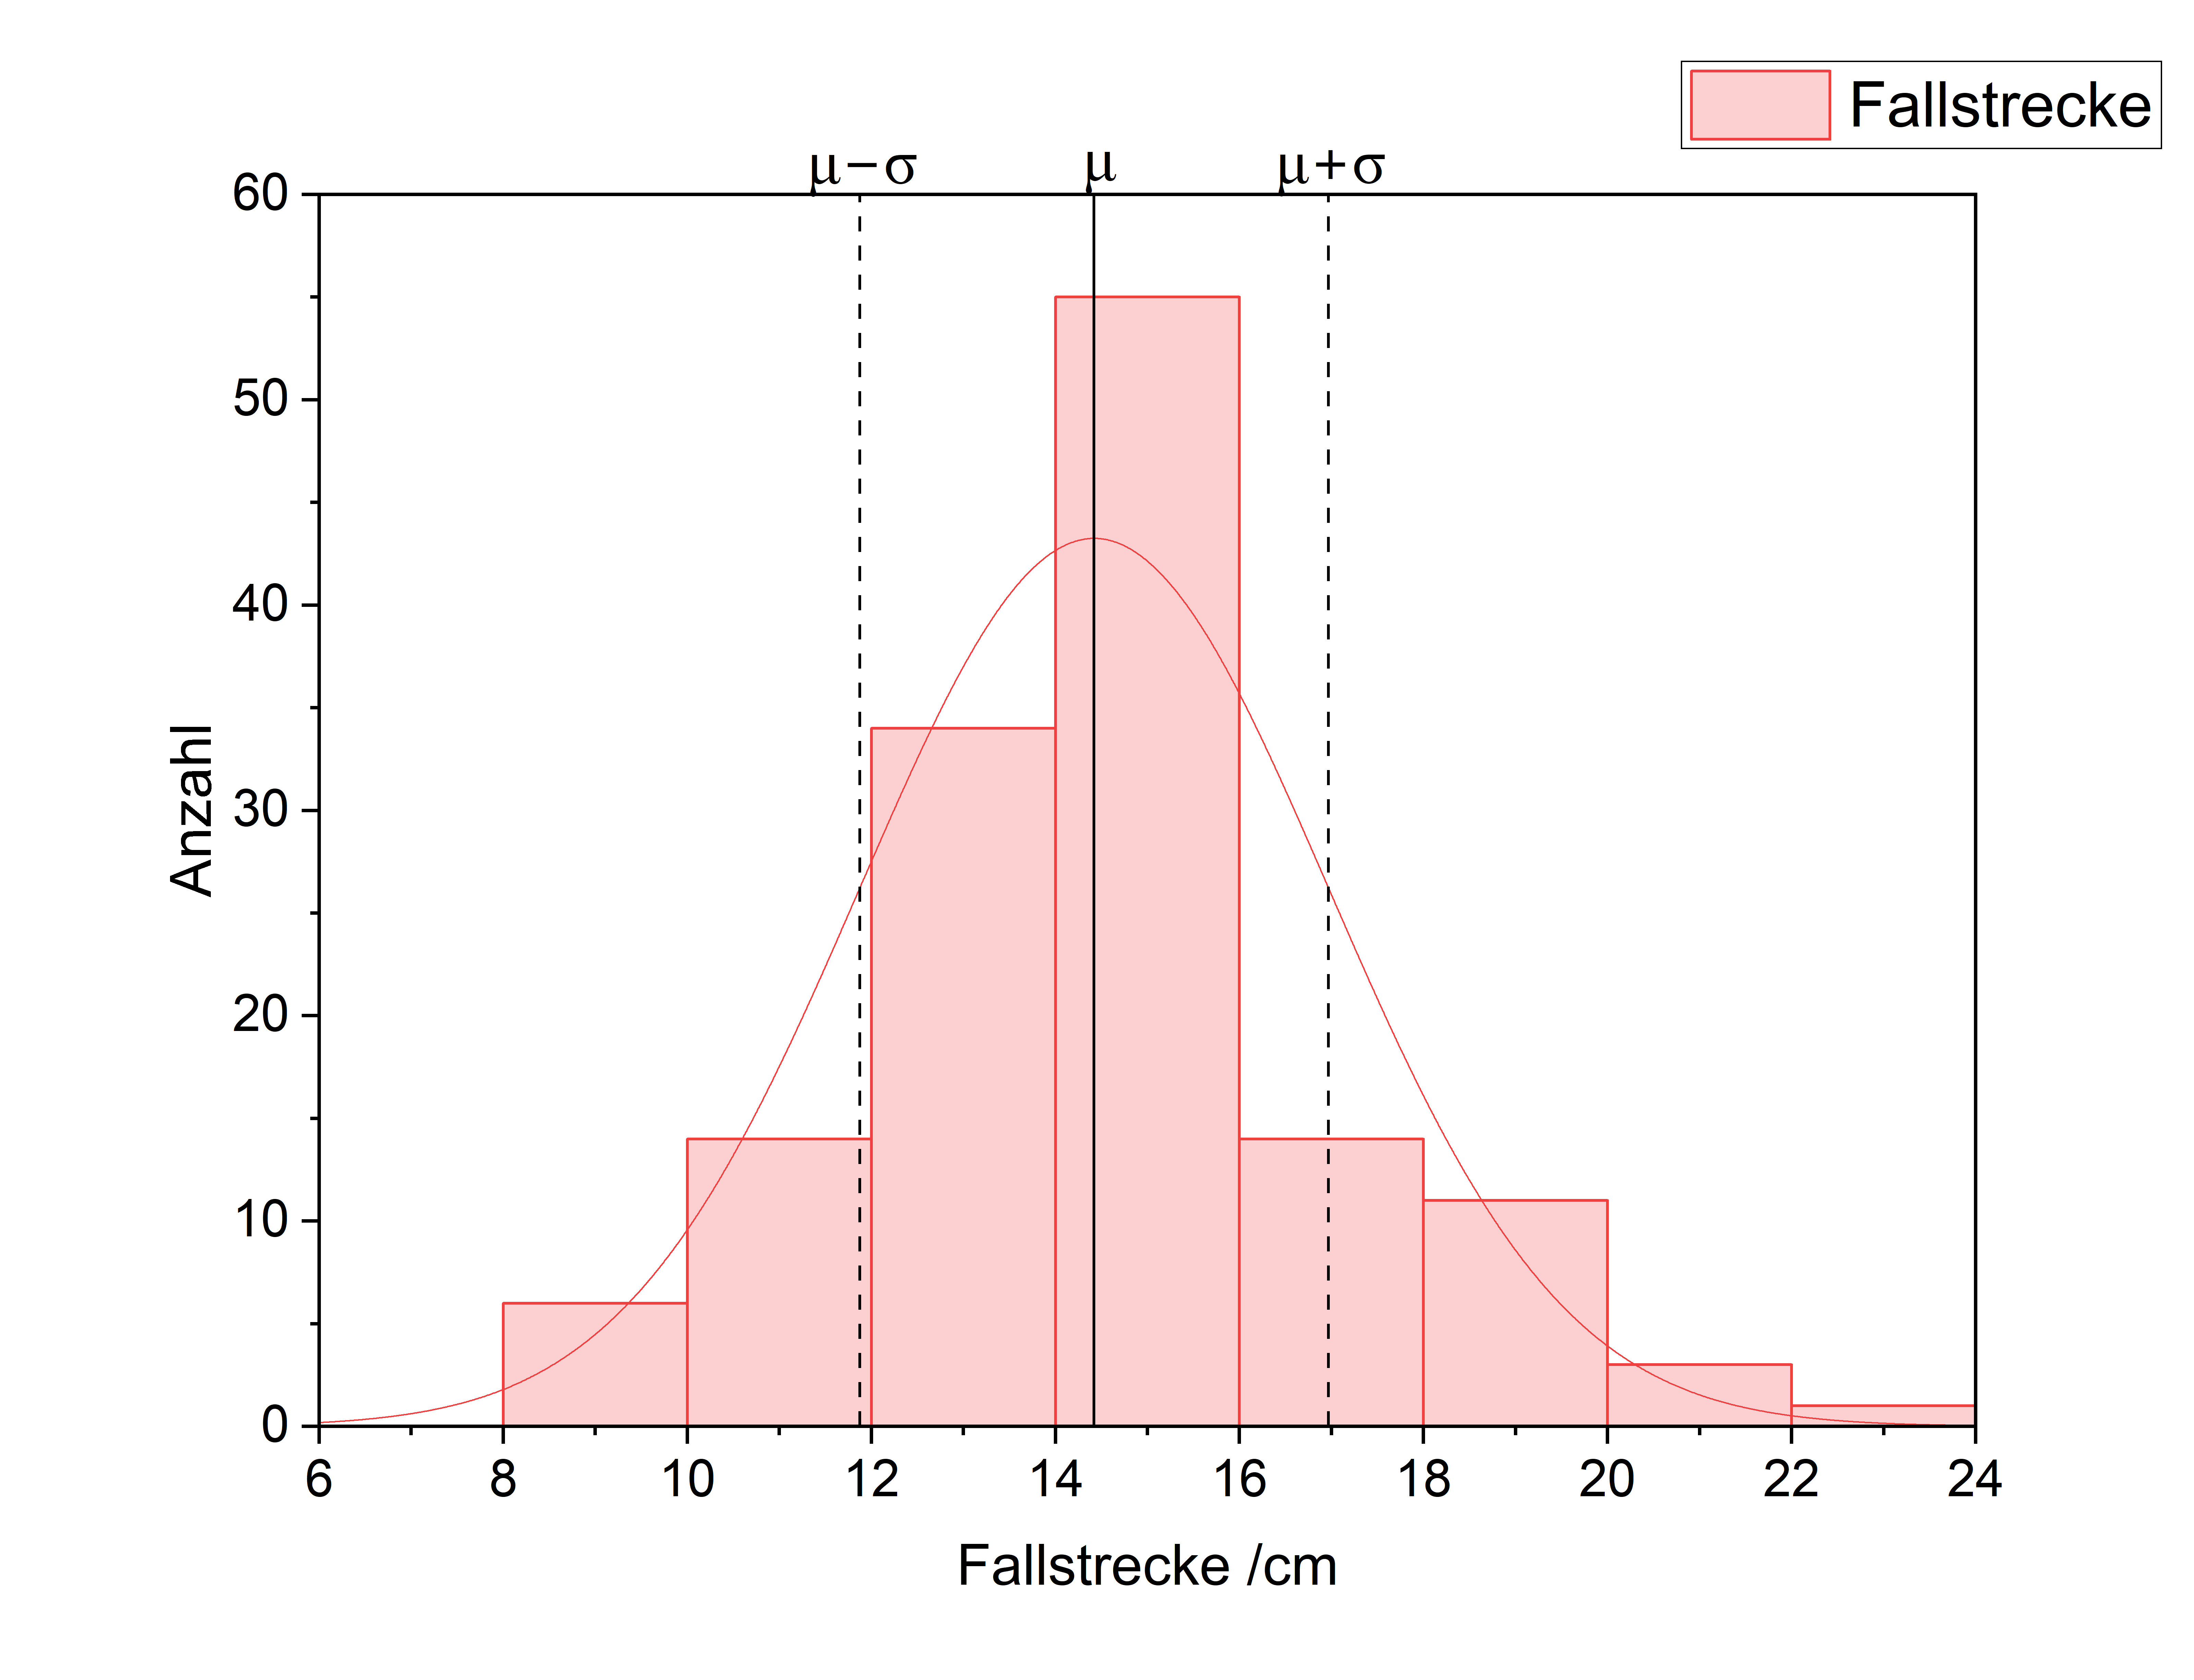
\includegraphics[width=15cm]{bilder/HistogrammFallstrecke.png}      %// [x] TODO: Diagramm Bild anpassen
    \caption{Histogramm der Fallstrecke}                                %// [x] TODO: Diagramm Bildunterschrift anpassen
\end{figure}

\vfill

\begin{figure}[H]
    \label{Abb:HistogrammReaktionszeit}
    \centering
    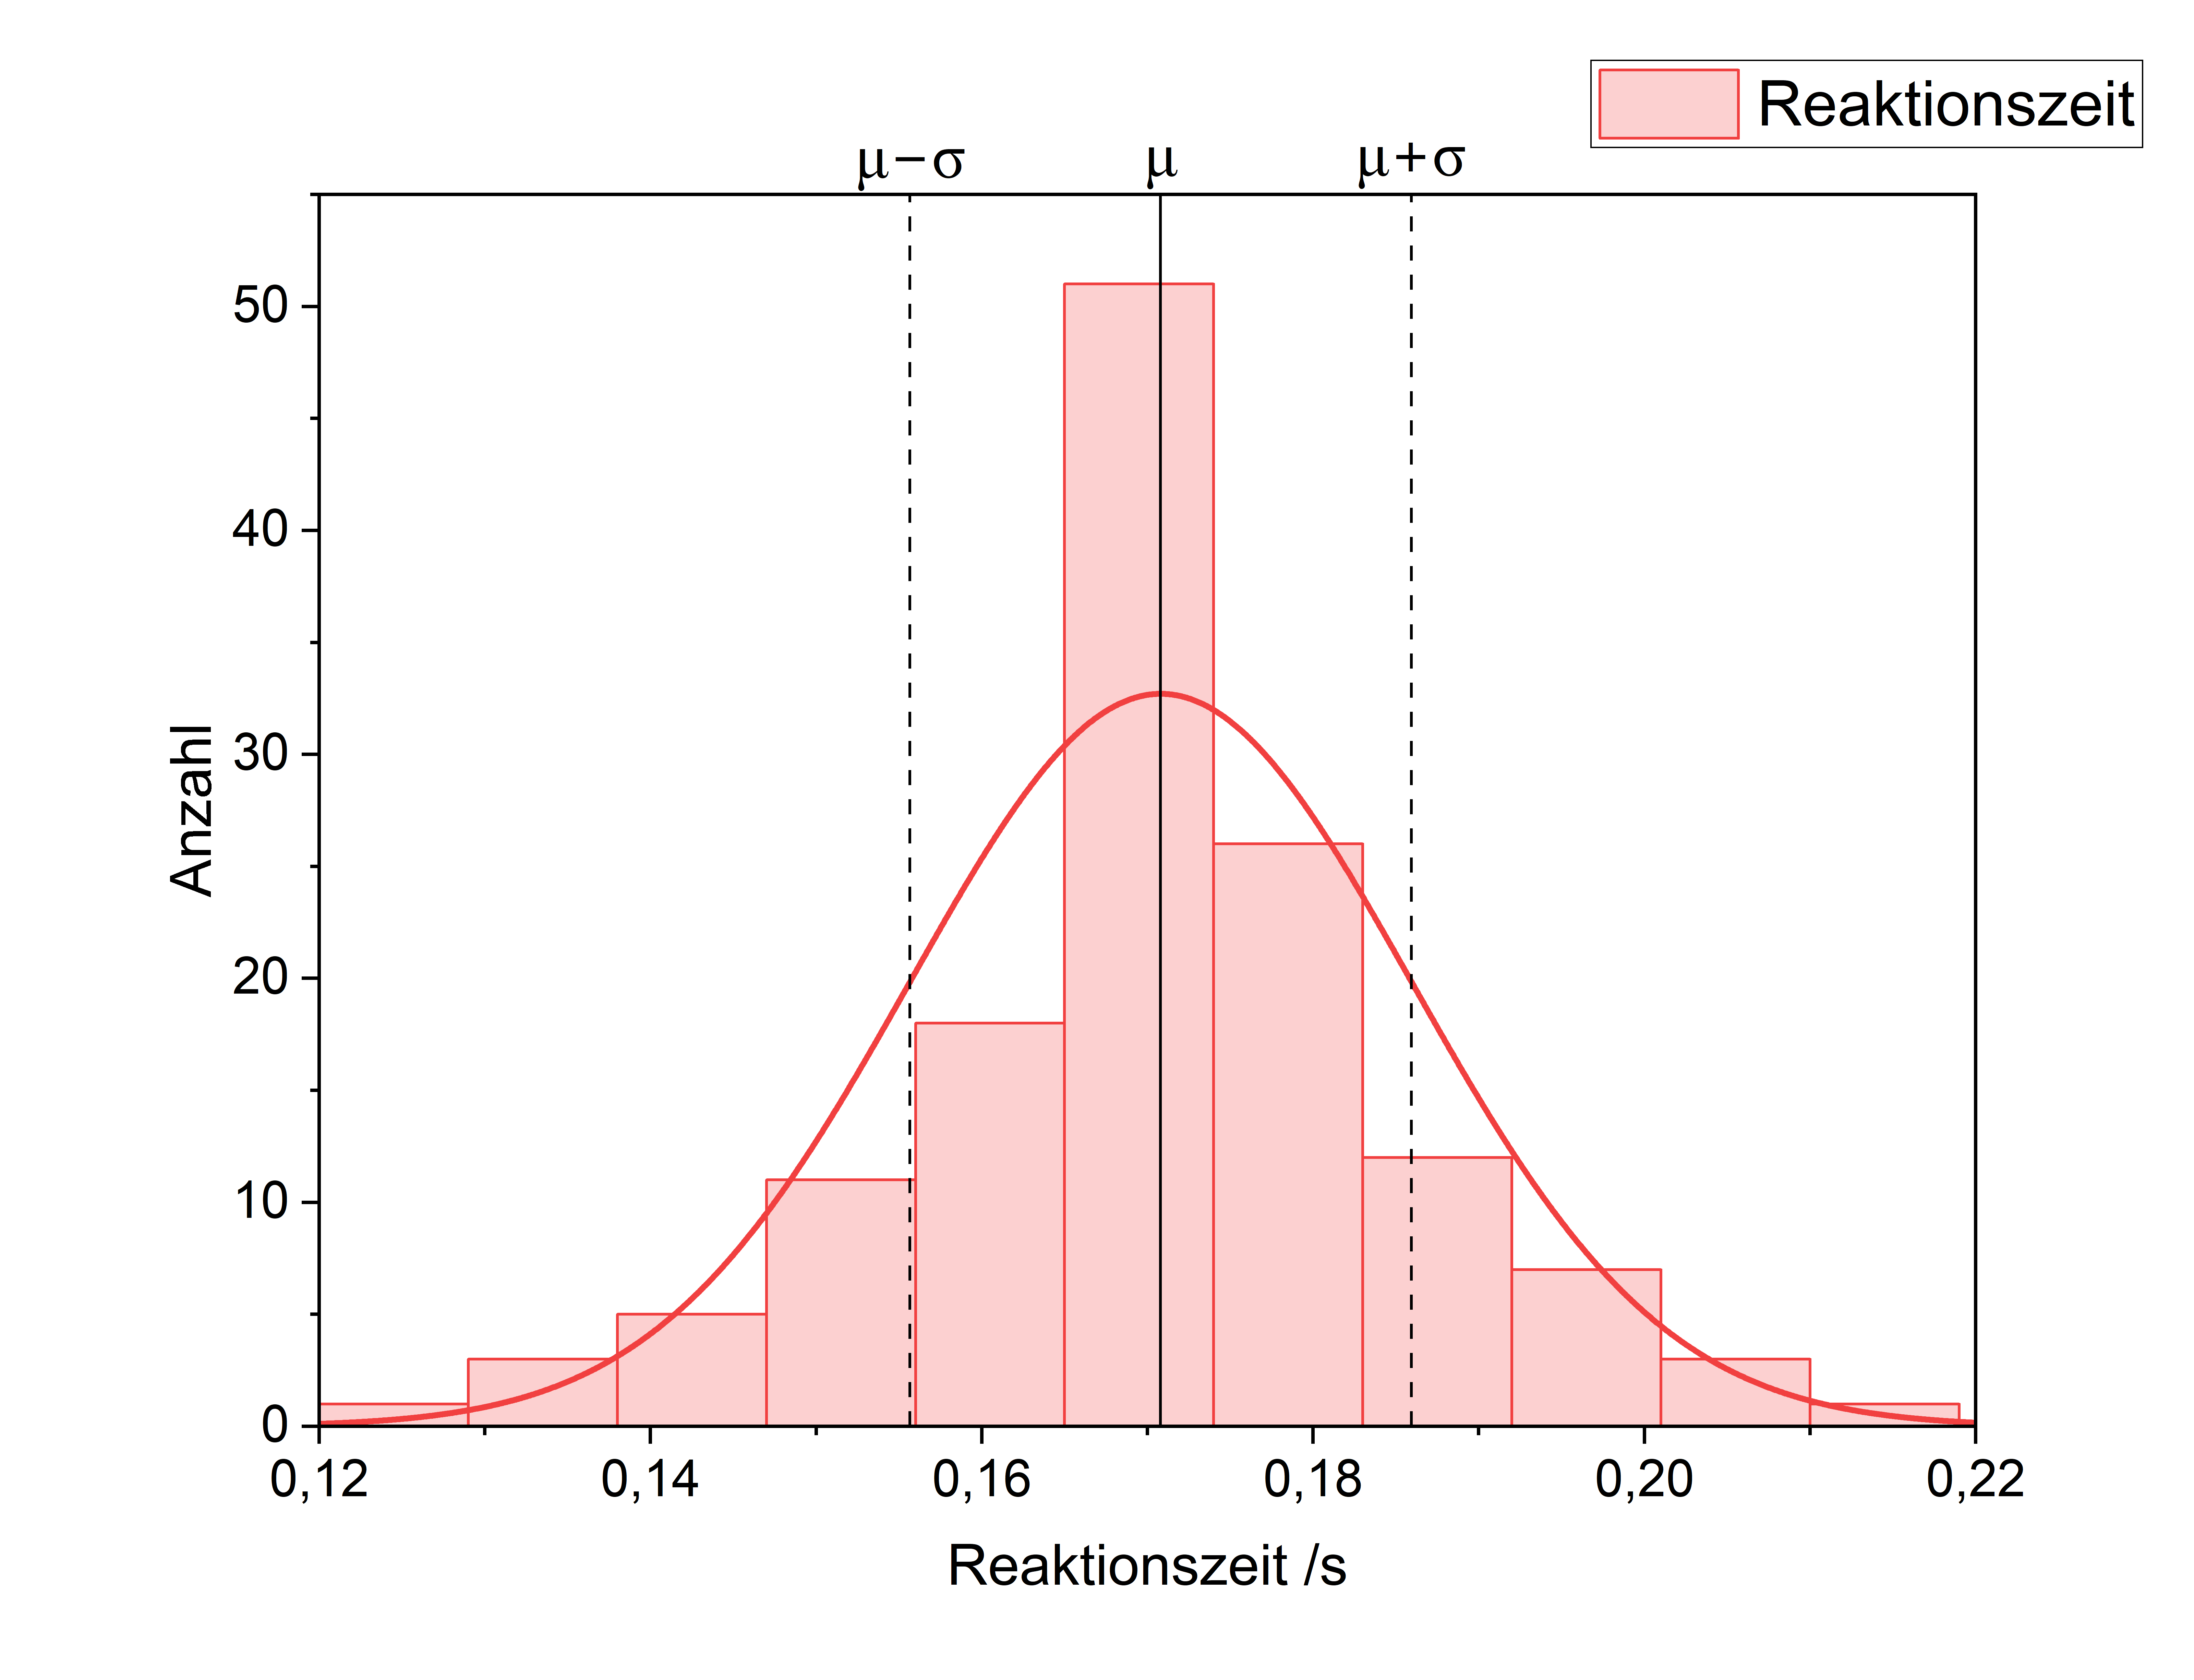
\includegraphics[width=15cm]{bilder/HistogrammReaktionszeit.png}    %// [x] TODO: Diagramm Bild anpassen
    \caption{Histogramm der Reaktionszeit}                              %// [x] TODO: Diagramm Bildunterschrift anpassen
\end{figure}


\section{Zusätzliche Messung der Reaktionszeit}

Zum Vergleich wird die Reaktionszeit von Eva Brandstätter mithilfe einer Stoppuhr gemessen.
Dabei werden auf der Anzeige alle, bis auf die erste Zehner-Ziffer der Sekundenanzeige verdeckt (Abb.
\ref{Abb:ZusatzversuchBild1}) und die Stoppuhr gestartet. Nach 10s erscheint eine 1 in der Anzeige
(Abb. \ref{Abb:ZusatzversuchBild2}), woraufhin so schnell wie möglich gestoppt wird. Danach wird
die Millisekundenanzeige als Wert für die Reaktionszeit abgelesen (Abb. \ref{Abb:ZusatzversuchBild3}).

\begin{multicols}{3}
    \begin{figure}[H]
        \centering
        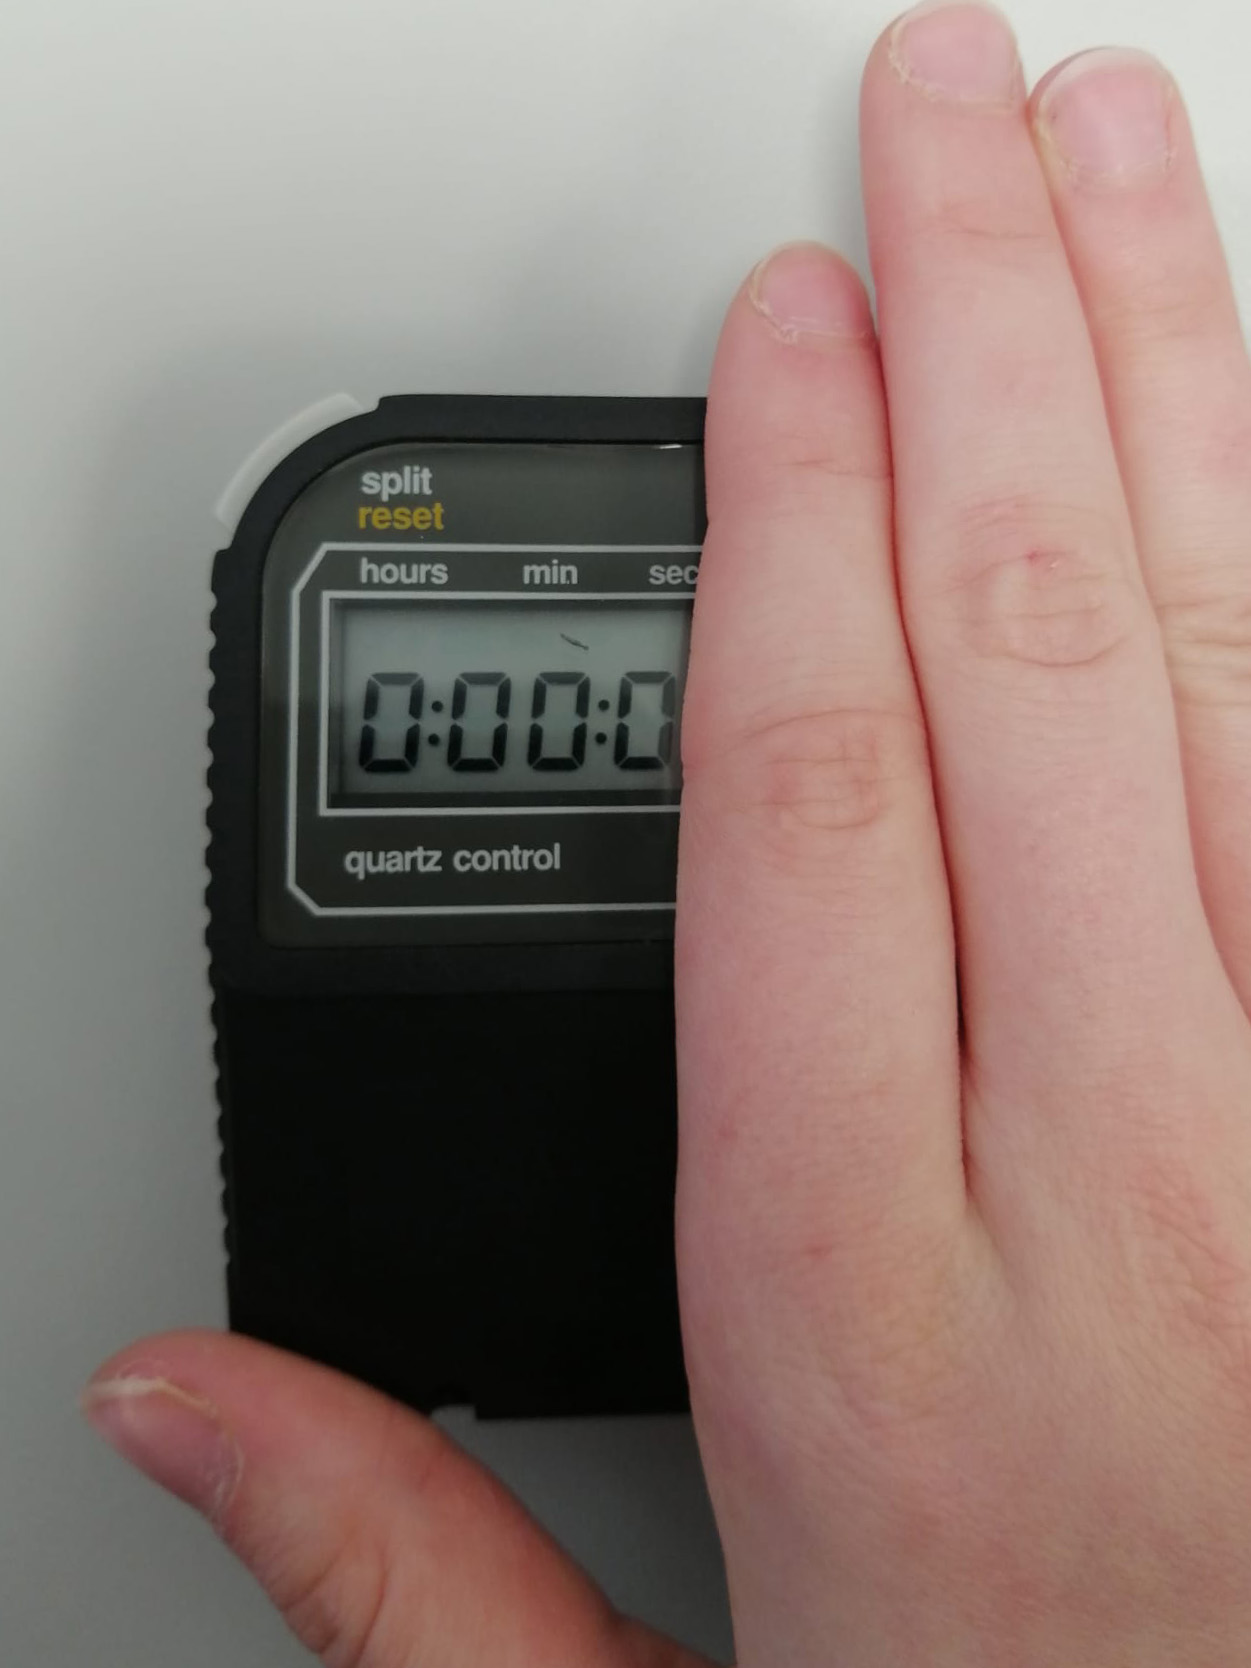
\includegraphics[width=5cm]{bilder/Zusatzversuch_1_export.jpg}
        \caption{\\Ausgangssituation}
        \label{Abb:ZusatzversuchBild1}
    \end{figure}
    \columnbreak
    \begin{figure}[H]
        \centering
        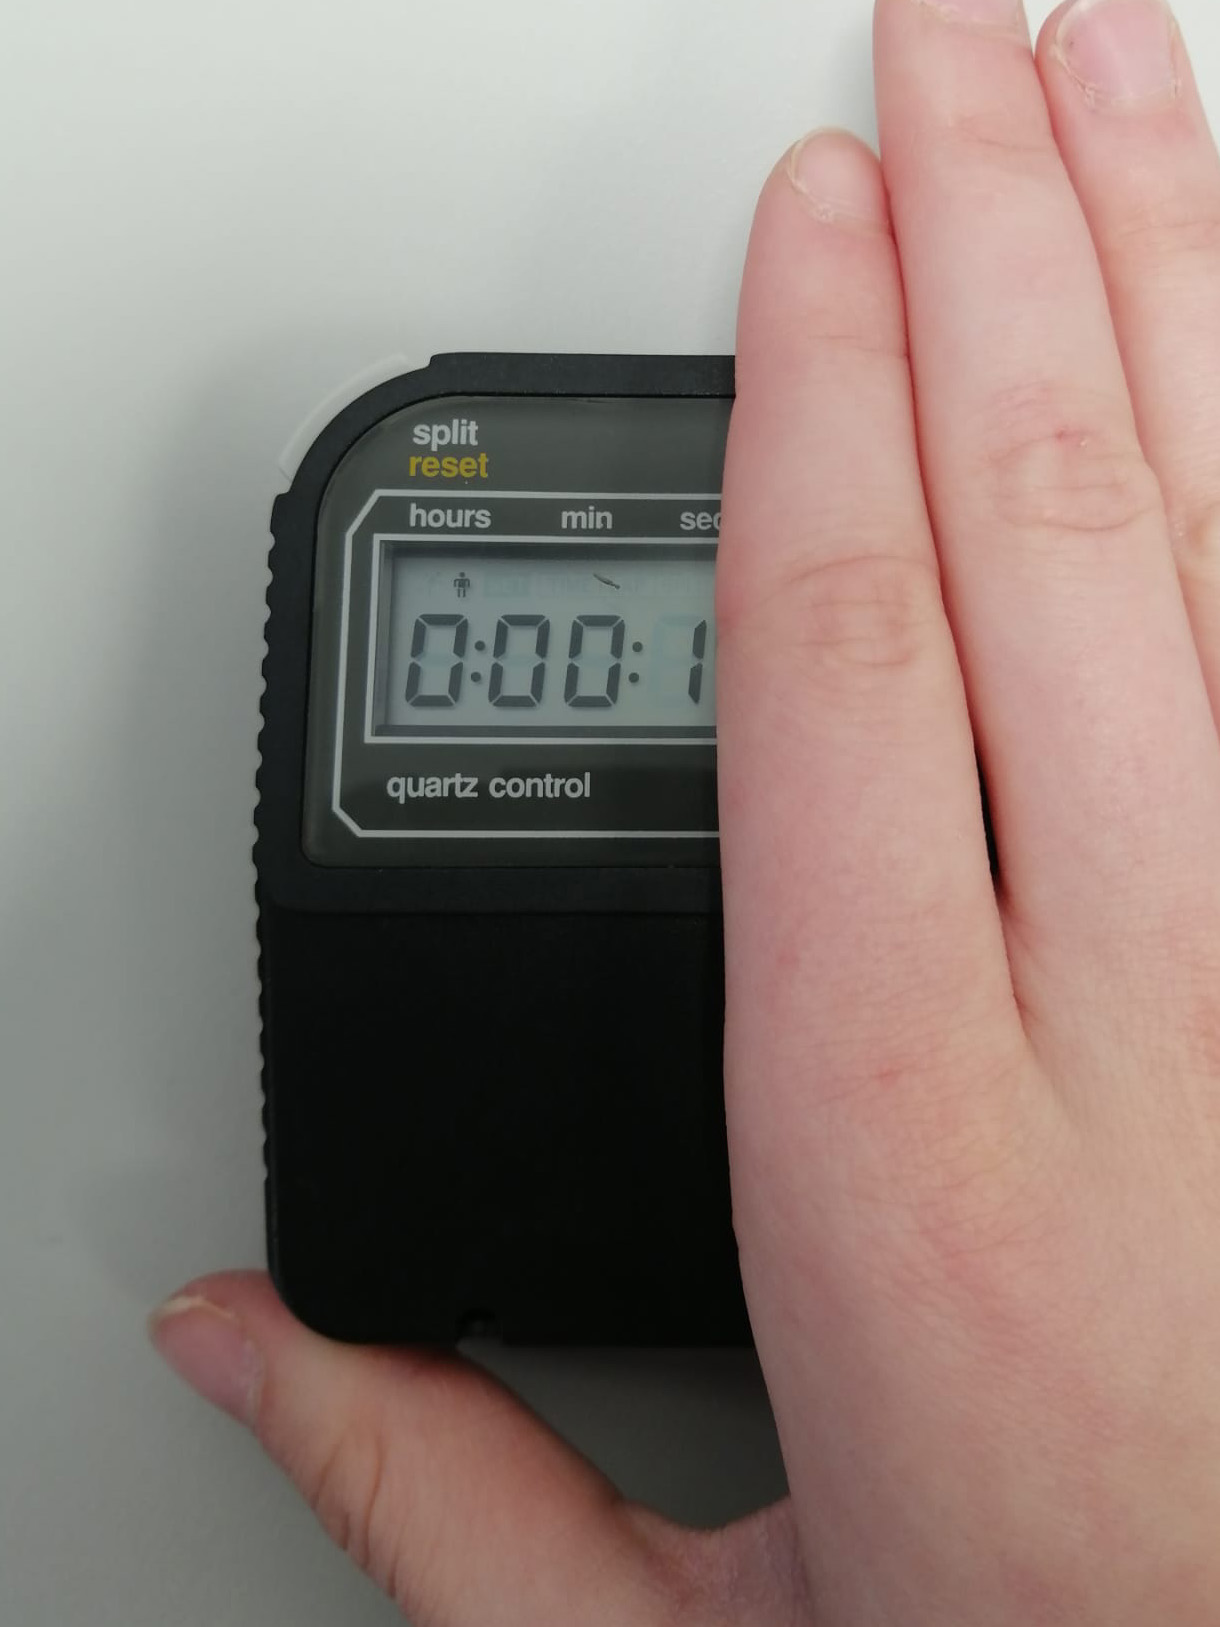
\includegraphics[width=5cm]{bilder/Zusatzversuch_2_export.jpg}
        \caption{\\auslösendes Ereignis}
        \label{Abb:ZusatzversuchBild2}
    \end{figure}
    \columnbreak
    \begin{figure}[H]
        \centering
        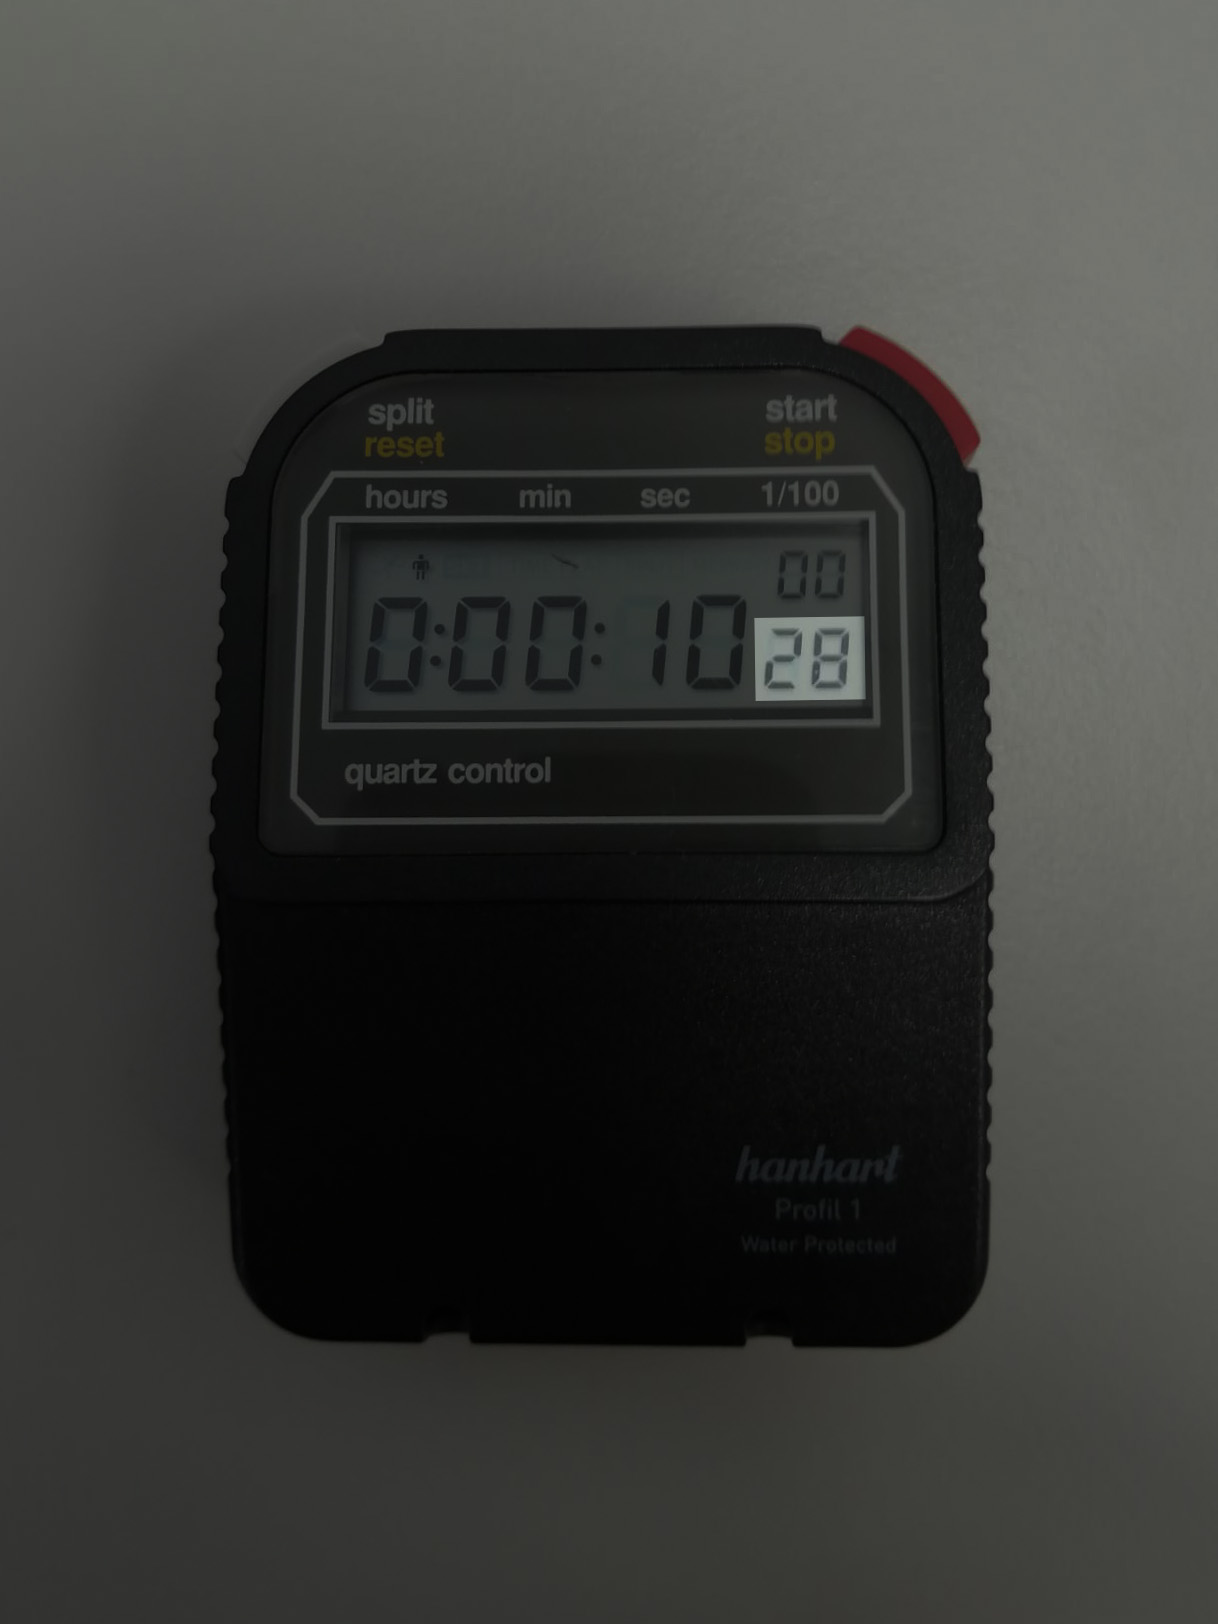
\includegraphics[width=5cm]{bilder/Zusatzversuch_3_export.jpg}
        \caption{Stoppuhr mit hervorgehobener Millisekundenanzeige}
        \label{Abb:ZusatzversuchBild3}
    \end{figure}
    \columnbreak
\end{multicols}

Dabei wurden für fünf Wiederholungen folgende Werte gemessen:

\begin{table}[H]
    \centering
    \label{Tab:StoppuhrVersuch}
    \begin{tabular}{|c|c|}
        \hline
        n & $t$ / $\mathrm{s}$ \\
        \hline
        1 & 0.280 \\
        2 & 0.280 \\
        3 & 0.220 \\
        4 & 0.250 \\
        5 & 0.250 \\
        \hline
    \end{tabular}
    \caption{Messwerte der Reaktionszeit mit Stoppuhr}
\end{table}


\section{Diskussion}
%//[ ] TODO: Diskussion
% Wie vergleicht sich meine Messung mit anderen Messungen/Theorien?
% Ist der Messwert sinnvoll? Stimmt die Größenordnung?
% Wo wurden Fehler gemacht? Was kann man verbessern?
% Gegebenenfalls rekursiv auswerten oder nachmessen!
% ursprüngliche Fragestellung diskutieren
% zB Standardabweichung diskutieren, berechnete Größen nennen

Die jeweils für Fallstrecke und Reaktionszeit berechneten Werte für Mittelwert, Standardabweichung und
Standardabweichung des Mittelwerts sind in einer sinnvollen Größenordnung und entsprechen weitgehend den Erwartungen.

Aus der Fehlerfortpflanzung ging hervor, dass für realistische Fallstrecken die Unsicherheit der Reaktionszeit
mit ca. $1$-$2\mathrm{ms}$ sehr gering ist.

Es wurde erkannt, dass $t(\mu_h)>\mu_t$ ist. Dies ist darauf zurückzuführen, dass die Verteilungsform
der Fallstrecke nicht mehr einer Normalverteilung entspricht, und eher nach links verzerrt ist.

Aus der Versuchsdurchführung wurden folgende Erkenntnisse gewonnen und Verbesserungsvorschläge abgeleitet:\\
Da die Zeit, die der Tester gewartet hat, bevor er das Lineal losgelassen hat, nicht dokumentiert wurde, 
kann nicht beurteilt werden, ob diese Zeit tatsächlich zufällig verteilt war, oder ob es eine unbewusste
Tendenz gab, bestimmte Zeiten zu wählen. Hätte man diese Zeit dokumentiert, könnte man daraus 
schließen, dass Ausreißerwerte in der Wartezeit eine deutliche Verschlechterung der Reaktionszeit der
Probandin zur Folge hätten.\\
Um auszuschließen, dass die Probandin noch nicht bereit war bzw. der Daumen noch nicht richtig ausgerichtet war,
wurde vereinbart, dass das Lineal erst nach einem Signal der Probandin losgelassen wird. Dadurch könnte die
Reaktionszeit verfälscht worden sein.\\
Außerdem sei erwähnt, dass die gemessenen Reaktionszeiten vermutlich im Zusammenhang mit der physischen
Verfassung der Probandin standen.

Weiters kann analysiert werden, ob es über die Dauer des Versuchs hinweg eine positive oder negative Tendenz im
Bezug auf die Reaktionszeit gab. Folgendes Diagramm (Abb. \ref{Abb:ReaktionszeitTendenz}) veranschaulicht, dass nur eine minimale Verschlechterung
festgestellt werden kann. Trotzdem wurde das Lineal von der fähigen Probandin nie fallengelassen.

\begin{figure}[H]
    \centering
    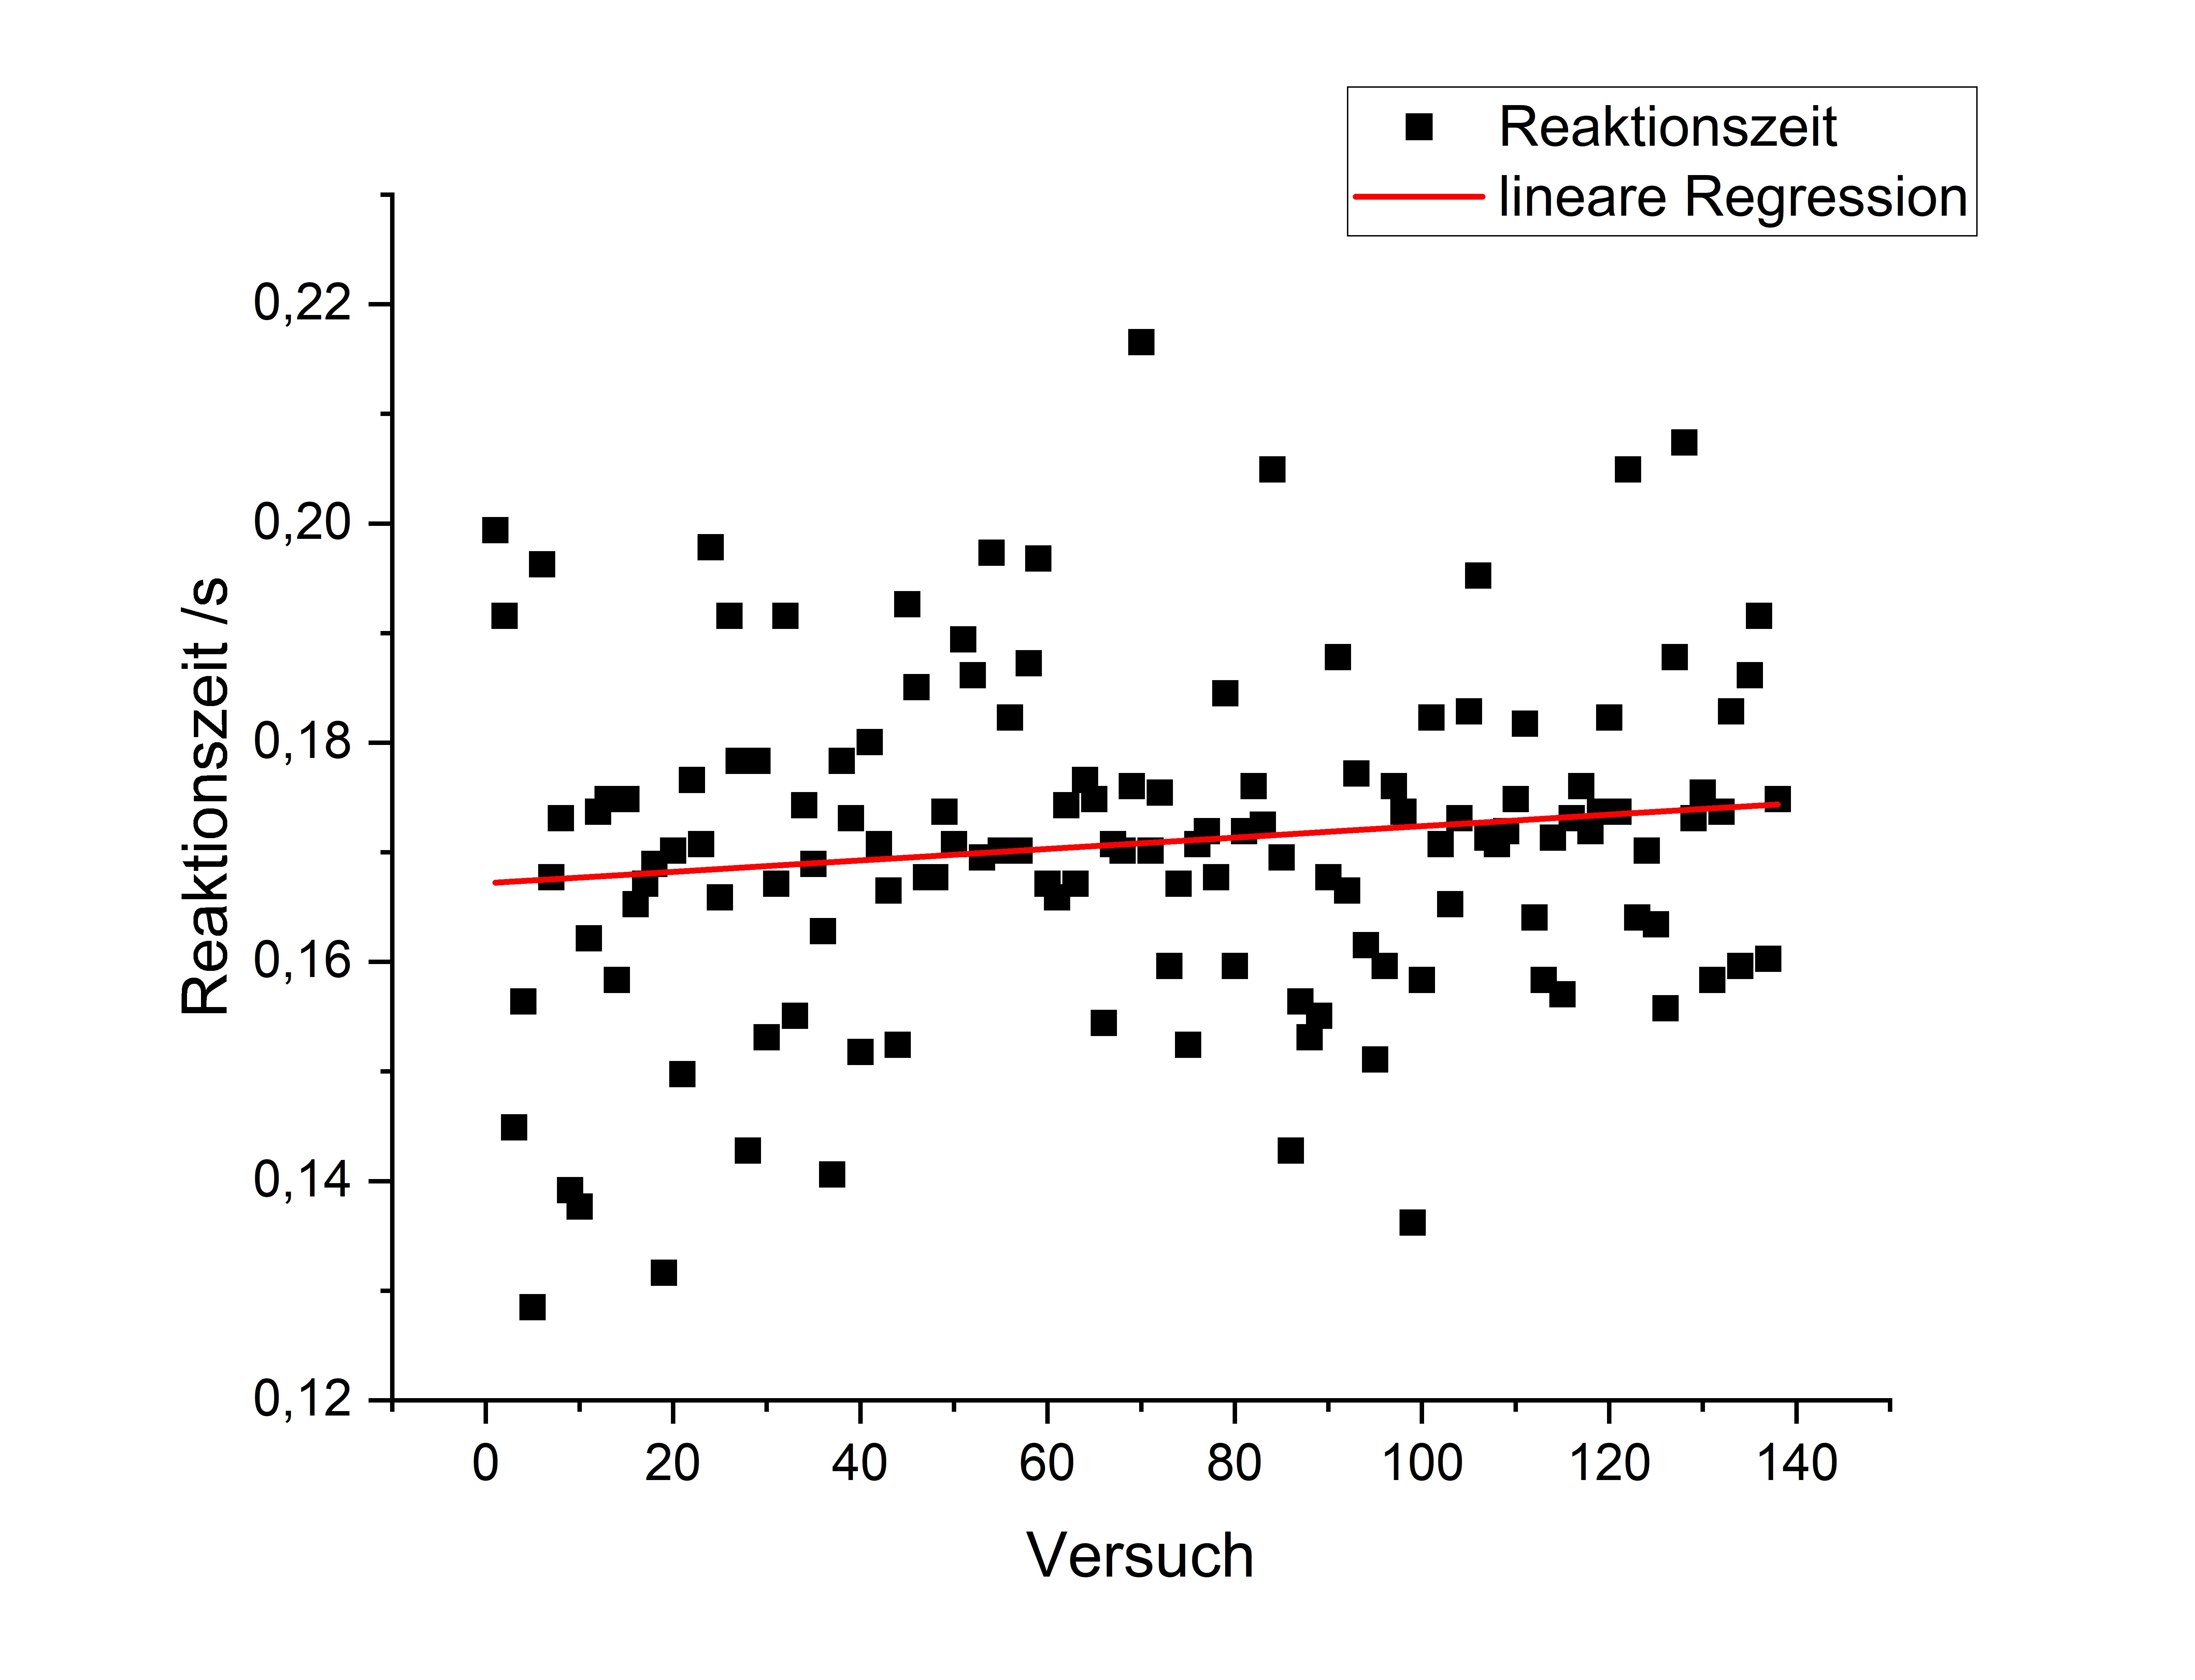
\includegraphics[width=13cm]{bilder/Tendenz1.png}          %// [x] TODO: Diagramm Bild anpassen
    \caption{Tendenz der Reaktionszeit}
    \label{Abb:ReaktionszeitTendenz}
\end{figure}

Um eine einen Vergleichswert für die aus den Fallstrecken ermittelte Reaktionszeit zu haben, wurde
eine zusätzliche direkte Reaktionszeitmessung mit einer Stoppuhr durchgeführt. Die gemessenen Werte
(Tab. \ref{Tab:StoppuhrVersuch}) liegen im Bereich von $0.220\mathrm{s}$ bis $0.280\mathrm{s}$ und
sind somit in einer ähnlichen Größenordnung, jedoch etwas höher als die aus den Fallstrecken ermittelten
Werte. Dies könnte auf mehrere Faktoren zurückzuführen sein, vor allem aber war der Stichprobenumfang
des Zusatzversuchs mit $n=5$ deutlich geringer und ist somit nur bedingt aussagekräftig.

Abschließend ist erwähnenswert, dass es wichtig ist, die Reaktionszeit zu kennen und zu verstehen,
da diese Einfluss auf andere Versuche und deren Ergebnisse haben kann.



\newpage
\section{Anhang}
\subsection{Fallstrecke \textit{h}}
\label{AnahangFallstrecke}

\begin{multicols}{4}

    \begin{table}[H]
        \centering
        \begin{tabular}{|c|r|}
            \hline
            & $h$ / $\mathrm{m}$ \\
            \hline
            1 & 19.5 \\
            2 & 18.0 \\
            3 & 10.3 \\
            4 & 12.0 \\
            5 & 8.1 \\
            6 & 18.9 \\
            7 & 13.8 \\
            8 & 14.7 \\
            9 & 9.5 \\
            10 & 9.3 \\
            11 & 12.9 \\
            12 & 14.8 \\
            13 & 15.0 \\
            14 & 12.3 \\
            15 & 15.0 \\
            16 & 13.4 \\
            17 & 13.7 \\
            18 & 14.0 \\
            19 & 8.5 \\
            20 & 14.2 \\
            21 & 11.0 \\
            22 & 15.3 \\
            23 & 14.3 \\
            24 & 19.2 \\
            25 & 13.5 \\
            26 & 18.0 \\
            27 & 15.6 \\
            28 & 10.0 \\
            29 & 15.6 \\
            30 & 11.5 \\
            31 & 13.7 \\
            32 & 18.0 \\
            33 & 11.8 \\
            34 & 14.9 \\
            35 & 14.0 \\
            \hline
        \end{tabular}
    \end{table}
    \columnbreak
    \begin{table}[H]
        \centering
        \begin{tabular}{|c|r|}
            \hline
            36 & 13.0 \\
            37 & 9.7 \\
            38 & 15.6 \\
            39 & 14.7 \\
            40 & 11.3 \\
            41 & 15.9 \\
            42 & 14.3 \\
            43 & 13.6 \\
            44 & 11.4 \\
            45 & 18.2 \\
            46 & 16.8 \\
            47 & 13.8 \\
            48 & 13.8 \\
            49 & 14.8 \\
            50 & 14.3 \\
            51 & 17.6 \\
            52 & 17.0 \\
            53 & 14.1 \\
            54 & 19.1 \\
            55 & 14.2 \\
            56 & 16.3 \\
            57 & 14.2 \\
            58 & 17.2 \\
            59 & 19.0 \\
            60 & 13.7 \\
            61 & 13.5 \\
            62 & 14.9 \\
            63 & 13.7 \\
            64 & 15.3 \\
            65 & 15.0 \\
            66 & 11.7 \\
            67 & 14.3 \\
            68 & 14.2 \\
            69 & 15.2 \\
            70 & 23.0 \\
            71 & 14.2 \\
            \hline
        \end{tabular}
    \end{table}
    \columnbreak
    \begin{table}[H]
        \centering
        \begin{tabular}{|c|r|}
            \hline
            72 & 15.1 \\
            73 & 12.5 \\
            74 & 13.7 \\
            75 & 11.4 \\
            76 & 14.3 \\
            77 & 14.5 \\
            78 & 13.8 \\
            79 & 16.7 \\
            80 & 12.5 \\
            81 & 14.5 \\
            82 & 15.2 \\
            83 & 14.6 \\
            84 & 20.6 \\
            85 & 14.1 \\
            86 & 10.0 \\
            87 & 12.0 \\
            88 & 11.5 \\
            89 & 11.8 \\
            90 & 13.8 \\
            91 & 17.3 \\
            92 & 13.6 \\
            93 & 15.4 \\
            94 & 12.8 \\
            95 & 11.2 \\
            96 & 12.5 \\
            97 & 15.2 \\
            98 & 14.8 \\
            99 & 9.1 \\
            100 & 12.3 \\
            101 & 16.3 \\
            102 & 14.3 \\
            103 & 13.4 \\
            104 & 14.7 \\
            105 & 16.4 \\
            106 & 18.7 \\
            107 & 14.4 \\
            \hline
        \end{tabular}
    \end{table}
    \columnbreak
    \begin{table}[H]
        \centering
        \begin{tabular}{|c|r|}
            \hline
            108 & 14.3 \\
            109 & 14.5 \\
            110 & 15.0 \\
            111 & 16.2 \\
            112 & 13.2 \\
            113 & 12.3 \\
            114 & 14.4 \\
            115 & 12.1 \\
            116 & 14.7 \\
            117 & 15.2 \\
            118 & 14.5 \\
            119 & 14.8 \\
            120 & 16.3 \\
            121 & 14.8 \\
            122 & 20.6 \\
            123 & 13.2 \\
            124 & 14.2 \\
            125 & 13.1 \\
            126 & 11.9 \\
            127 & 17.3 \\
            128 & 21.1 \\
            129 & 14.7 \\
            130 & 15.1 \\
            131 & 12.3 \\
            132 & 14.8 \\
            133 & 16.4 \\
            134 & 12.5 \\
            135 & 17.0 \\
            136 & 18.0 \\
            137 & 12.6 \\
            138 & 15.0 \\
            \hline
        \end{tabular}
        \caption{Fallstrecke}
    \end{table}
    
\end{multicols}


\newpage
\subsection{Reaktionszeit \textit{t}}
\label{AnahangReaktionszeit}

\begin{multicols}{4}

    \begin{table}[H]
        \centering
        \begin{tabular}{|c|r|}
            \hline
            & $t$ / $\mathrm{s}$ \\
            \hline
            1   & 0.1994 \\
            2   & 0.1916 \\
            3   & 0.1449 \\
            4   & 0.1564 \\
            5   & 0.1285 \\
            6   & 0.1963 \\
            7   & 0.1677 \\
            8   & 0.1731 \\
            9   & 0.1392 \\
            10  & 0.1377 \\
            11  & 0.1622 \\
            12  & 0.1737 \\
            13  & 0.1749 \\
            14  & 0.1584 \\
            15  & 0.1749 \\
            16  & 0.1653 \\
            17  & 0.1671 \\
            18  & 0.1689 \\
            19  & 0.1316 \\
            20  & 0.1701 \\
            21  & 0.1498 \\
            22  & 0.1766 \\
            23  & 0.1707 \\
            24  & 0.1978 \\
            25  & 0.1659 \\
            26  & 0.1916 \\
            27  & 0.1783 \\
            28  & 0.1428 \\
            29  & 0.1783 \\
            30  & 0.1531 \\
            31  & 0.1671 \\
            32  & 0.1916 \\
            33  & 0.1551 \\
            34  & 0.1743 \\
            35  & 0.1689 \\
            \hline
        \end{tabular}
    \end{table}
    \columnbreak
    \begin{table}[H]
        \centering
        \begin{tabular}{|c|r|}
            \hline
            36  & 0.1628 \\
            37  & 0.1406 \\
            38  & 0.1783 \\
            39  & 0.1731 \\
            40  & 0.1518 \\
            41  & 0.1800 \\
            42  & 0.1707 \\
            43  & 0.1665 \\
            44  & 0.1525 \\
            45  & 0.1926 \\
            46  & 0.1851 \\
            47  & 0.1677 \\
            48  & 0.1677 \\
            49  & 0.1737 \\
            50  & 0.1707 \\
            51  & 0.1894 \\
            52  & 0.1862 \\
            53  & 0.1695 \\
            54  & 0.1973 \\
            55  & 0.1701 \\
            56  & 0.1823 \\
            57  & 0.1701 \\
            58  & 0.1873 \\
            59  & 0.1968 \\
            60  & 0.1671 \\
            61  & 0.1659 \\
            62  & 0.1743 \\
            63  & 0.1671 \\
            64  & 0.1766 \\
            65  & 0.1749 \\
            66  & 0.1544 \\
            67  & 0.1707 \\
            68  & 0.1701 \\
            69  & 0.1760 \\
            70  & 0.2165 \\
            71  & 0.1701 \\
            \hline
        \end{tabular}
    \end{table}
    \columnbreak
    \begin{table}[H]
        \centering
        \begin{tabular}{|c|r|}
            \hline
            72  & 0.1755 \\
            73  & 0.1596 \\
            74  & 0.1671 \\
            75  & 0.1525 \\
            76  & 0.1707 \\
            77  & 0.1719 \\
            78  & 0.1677 \\
            79  & 0.1845 \\
            80  & 0.1596 \\
            81  & 0.1719 \\
            82  & 0.1760 \\
            83  & 0.1725 \\
            84  & 0.2049 \\
            85  & 0.1695 \\
            86  & 0.1428 \\
            87  & 0.1564 \\
            88  & 0.1531 \\
            89  & 0.1551 \\
            90  & 0.1677 \\
            91  & 0.1878 \\
            92  & 0.1665 \\
            93  & 0.1772 \\
            94  & 0.1615 \\
            95  & 0.1511 \\
            96  & 0.1596 \\
            97  & 0.1760 \\
            98  & 0.1737 \\
            99  & 0.1362 \\
            100 & 0.1584 \\
            101 & 0.1823 \\
            102 & 0.1707 \\
            103 & 0.1653 \\
            104 & 0.1731 \\
            105 & 0.1829 \\
            106 & 0.1953 \\
            107 & 0.1713 \\
            \hline
        \end{tabular}
    \end{table}
    \columnbreak
    \begin{table}[H]
        \centering
        \begin{tabular}{|c|r|}
            \hline
            108 & 0.1707 \\
            109 & 0.1719 \\
            110 & 0.1749 \\
            111 & 0.1817 \\
            112 & 0.1640 \\
            113 & 0.1584 \\
            114 & 0.1713 \\
            115 & 0.1571 \\
            116 & 0.1731 \\
            117 & 0.1760 \\
            118 & 0.1719 \\
            119 & 0.1737 \\
            120 & 0.1823 \\
            121 & 0.1737 \\
            122 & 0.2049 \\
            123 & 0.1640 \\
            124 & 0.1701 \\
            125 & 0.1634 \\
            126 & 0.1558 \\
            127 & 0.1878 \\
            128 & 0.2074 \\
            129 & 0.1731 \\
            130 & 0.1755 \\
            131 & 0.1584 \\
            132 & 0.1737 \\
            133 & 0.1829 \\
            134 & 0.1596 \\
            135 & 0.1862 \\
            136 & 0.1916 \\
            137 & 0.1603 \\
            138 & 0.1749 \\
            \hline
        \end{tabular}
        \caption{\\Reaktionszeit}
    \end{table}
    
\end{multicols}


\end{document}

% unsicherheit der zeit zu jeder zeit dazuschreiben
